% CAPITOLO LITERATURE REVIEW
\newpage
\section{Literature Review}
\label{section:literatureReviewChapter}
This chapter provides an in-depth look at the field of generative modelling. It lays out the theoretical background of the thesis, beginning with a general explanation of the workings of GANs and then delving into the concepts behind specific GANs that are utilised to achieve the ultimate objective of the study.

\subsection{GAN}
The innovative concept of Generative Adversarial Networks (GANs) was first introduced in 2014 by Goodfellow and his colleagues from the University of Montreal \cite{GANGoodfellow}. GANs are a type of deep learning model that has the ability to generate new content, such as text or images, based on a given dataset. GANs have been the focus of significant research in recent years and have made significant contributions to the field of computer vision. The technology has advanced in areas like generating realistic images, transforming images, modifying facial features, and similar areas, but also in other areas such as music generation.\\
Before the advent of GANs, machine learning algorithms were highly effective in recognising patterns in existing data and could be utilised for tasks like classification and prediction. However, generating new data presented a challenge for these algorithms. The solution proposed in the GAN paper leverages the strengths of machine learning algorithms — their ability to classify and predict – to overcome their weaknesses in generating new content.\\
The approach involves setting two algorithms against each other in a kind of competition, leading to a continuous process of improvement. This approach has proven to be highly effective in generating new, diverse content and has been widely adopted in the field of deep learning.
Before diving into the intricacies of GANs, it is essential to understand how these networks work. A widely used analogy can provide a clearer insight.\\
\\
Imagine there is an art forger and an art authenticator. The forger's goal is to produce a counterfeit piece of art that the authenticator will consider genuine. The authenticator is trained to recognise genuine art by examining real pieces, while the forger learns by creating art that is then evaluated by the authenticator. In GANs, the forger is the generator, which strives to produce examples that are indistinguishable from the real data in the training set, thus trying to fool the discriminator. On the other hand, the discriminator acts as the art authenticator, evaluating the authenticity of the generated pieces. These two networks are in a constant battle, each trying to outsmart the other. As the generator improves in creating realistic data, the discriminator needs to enhance its capability in detecting fake examples. Similarly, as the discriminator becomes better at telling true from false, the generator must strive to generate even more convincing fake data. The most critical aspect of this architecture is that the generator has no direct connection to the actual image. The only way of learning of the generator is through its interaction with the discriminator \cite{GeneratingNewRealityBook}. Fig. \ref{fig:GAN architecture} illustrates a simple GAN architecture based on the analogy.
\begin{figure}[h!]
\centering
  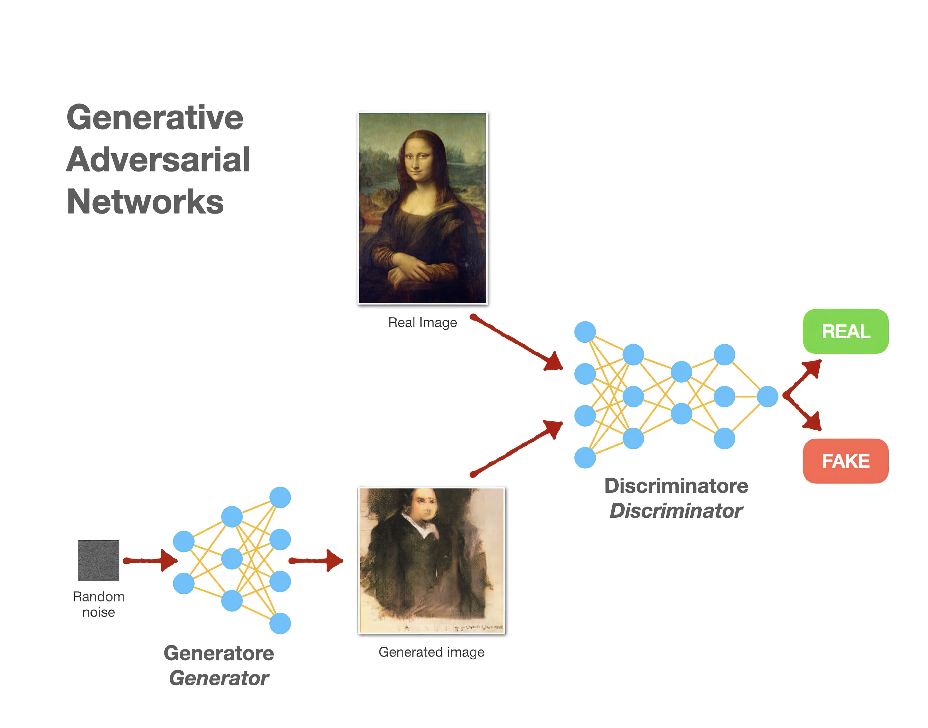
\includegraphics[scale=0.5]{figures/GANs-ex-art.png}
  \caption{Example of a GAN architecture}
  \label{fig:GAN architecture}
\end{figure}

\subsubsection{GAN structure and training}
\noindent A GAN has a similar structure to that of an autoencoder, where the discriminator serves as the encoder. However, instead of producing an encoded representation, it only outputs whether the input is real or fake. On the other hand, the generator acts like the decoder and takes in random data from the latent space, learning to generate new content that can trick the discriminator into thinking it is real. Both the generator and discriminator are trained in a competitive manner, with the generator striving to maximise the error of the discriminator and the discriminator trying to minimise it.\\
\\
The generator and the discriminator are two distinct deep neural networks. The generator is a function G that takes random noise vector $z$ as inputs and maps them to the data space, producing a set of synthetic samples. These samples are fed into the discriminator network D, together with the real samples $x$. This network outputs a single scalar that represents the probability that the sample came from the real data distribution rather than the synthetic data distribution. Therefore, the discriminator learns to use traditional supervised learning techniques, dividing inputs into two classes (real or fake).\\
The GAN training process is a two-player that involves updating the weights of the generator and discriminator networks using gradients computed from the loss function. The loss function, also called cost function, in a GAN is designed to quantify the difference between the generated data and the real data. The objective is to find the balance between the generator and discriminator losses, where the generator loss represents the ability of the generator to produce realistic synthetic data and the discriminator loss represents the ability of the discriminator to distinguish between real and fake data.\\
There are several cost functions that may be used, and they usually differ in terms of the cost function used for the generator.\\
The basic loss function used in GAN is the binary cross-entropy:
\begin{equation}
\label{eq:binariCross-entropy}
L(\hat{y}, y) = [y \times \log (\hat{y}) + (1-y)\times \log (1-\hat{y})]
\end{equation}
where $y$ represent the original data and $\hat{y}$ the generated one. In training the discriminator it is assumed $y=1$ for real data, while for the generated it is set: $\hat{y} = D(x)$. Substituting this information in equation \ref{eq:binariCross-entropy} it can be obtained the discriminator loss: 
\begin{equation}
    L(D(x),1)=\log(D(x))
\end{equation}
For the generator's output data it is assumed $y = 0$, because it outputs fake data, and $\hat{y} = G(D(z))$ for the generated data, where $z$ is a random noise vector sampled from a noise distribution $p_z(z)$ (e.g., uniform or Gaussian distribution). Therefore, the loss for the generator is:
\begin{equation}
    L(D(G(z)),0) = \log(1 - D(G(z)))
\end{equation}
To obtain the total discriminator loss the two above equations have to be combined and maximised:
\begin{equation}
L^{(D)}=\max [\log (D(x)) + \log(1-D(G(z)))]
\end{equation}
The generator has the opposite goal, therefore to obtain its loss function is obtaining by computing the minimum:
\begin{equation}
L^{(G)}=\min [\log (D(x)) + \log(1-D(G(z)))]
\end{equation}
The discriminator loss is defined as the log-likelihood of assigning the correct label to both real data and generated data. This loss function is designed to encourage the generator to produce realistic synthetic data and the discriminator to distinguish between real and fake data with high accuracy. While, the generator loss is usually defined as the log-likelihood of the discriminator assigning the correct label (real or fake) to the generated data.
\\
The interdependence of each player's cost on the other player's parameters, along with the lack of control over the other player's parameters, makes this scenario more accurately described as a game rather than an optimisation problem.
The loss function in a GAN is an important component of the training process, as it determines the quality of the generated data and the ability of the discriminator to accurately distinguish between real and fake data. 
\\
\noindent The training process of GANs is a zero-sum game in which the objective function of this minimax optimisation problem is:
\begin{equation}
    \min \max V(D,G) = \min_G \max_D E_{x \sim p_{data}(x)}[\log D(x)]+E_{z \sim p_z(z)}[\log (1- D(G(z)))]
\end{equation}
where $x$ is a real image from the true data distribution $p_{data}$, and $z$ is a noise vector sampled from the prior distribution $p_z$.

\noindent In training a GAN, it is important to ensure that both the generator and discriminator models are developed in a balanced manner. The success of the GAN largely depends on the alignment of the real and generated distributions, and this can only be achieved if neither of the models is overly dominant. If the discriminator is too good at identifying fake versus real images early in the training process, the generator may struggle to produce convincing fake images, making it difficult for the two models to improve. It is therefore crucial to establish a balanced relationship between the generator and discriminator models, allowing them to train efficiently and effectively.\\
If the generator is successful in fooling the discriminator, the loss will backpropagate through the discriminator network to improve its performance. On the other hand, if the discriminator is successful in classifying fake and real samples, the loss will backpropagate through the generator network to improve its ability to generate samples that are similar to real samples. If the discriminator is too effective at separating fake from real examples early on, the generator's task becomes extremely difficult. \\ 
From a mathematical point of view, if the discriminator gets too better at identifying the samples, this may increase the divergence between the generated expected distribution. In case the generated and the real distributions become too diverse or do not overlap, then the generator will suffer from vanishing gradient loss. \\
The vanishing gradient problem is a common issue in training deep neural networks. The problem occurs when the gradients of the parameters with respect to the loss become extremely small, making it difficult for the optimizer to update the parameters of the network effectively since they have no effect on the training model. The vanishing gradient problem is a critical issue in training deep neural networks and can lead to slow convergence or complete failure of the training process. The goal is to make the expected and generated distribution match as closely as possible. 
The GAN continues this back and forth process until an equilibrium is reached between the generator and discriminator loss. Over time, the two networks learn from each other and converge to a state where the generator produces samples that are almost indistinguishable from real data, and the discriminator is able to correctly identify which samples are real and which are fake with high accuracy \cite{GANGoodfellow, GeneratingNewRealityBook}.
 \\
This basic design is referred to as the Vanilla GAN, as it represents the original model from which more advanced GAN architectures have evolved, yet still retaining the two key components of the GAN structure.


% ************************************
\subsection{ProGAN}
ProGAN, short for Progressive Generative Adversarial Network, is a deep learning model that was developed to generate high-resolution, photorealistic images. It was introduced by Karras et al. in 2017 \cite{ProGAN}, it is a type of generative model, which means that it can generate new, synthetic images based on the data it was trained on.\\
The main idea behind ProGAN is to use a series of generators and discriminators to generate high-resolution images incrementally, starting from low-resolution images (e.g. 4×4) and gradually increasing the resolution until a high-resolution image is obtained (e.g. 1024×1024). This approach is called progressive growing, and it allows the network to learn the finer details of an image in an incremental manner. The generator starts with a random noise input and generates an image with low resolution, which is then evaluated by the discriminator. The discriminator determines whether the generated image is real or not and provides feedback to the generator, allowing it to improve. \\ \\
One of the benefits of ProGAN is that it generates high-resolution images that are photorealistic, which makes it useful for various applications. Additionally, ProGAN is trained on large datasets, which means that it can generate diverse and varied images.
Another advantage of ProGAN is its ability to generate images at different resolutions, which allows for a level of control over the generated images. \\ The drawback of the progressive growth method in a GAN is the prolonged training time involved in constructing subsequent models at higher resolutions, it also requires extra resources in terms of data preparation and storage, and of course a non-negligible computational time.

